\documentclass[11pt]{standalone}

\usepackage{ifthen}
\usepackage{tikz} 
\usetikzlibrary{shapes.misc}
\usetikzlibrary{arrows,arrows.meta}
\usetikzlibrary{calc,intersections, patterns, math}

\definecolor{pfeil}{RGB}{168,167,167}
\definecolor{bg}{RGB}{23,23,23}
\definecolor{petrol}{RGB}{0, 118, 136}
\definecolor{darkgoldenrod}{RGB}{184, 134, 11}
\colorlet{petrol-lighter}{petrol!40}
\colorlet{darkgoldenrod-lighter}{darkgoldenrod!40}

\begin{document}

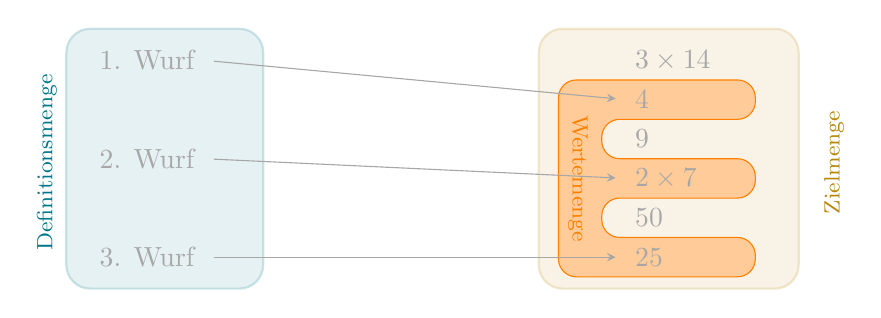
\begin{tikzpicture}[pfeil]

    \draw[thick, fill=petrol!20, draw=petrol-lighter, rounded corners=2ex, opacity=0.5] (-1,0.1) rectangle ++ (2.5,3.3);
    \draw[thick, fill=darkgoldenrod!20, draw=darkgoldenrod-lighter, rounded corners=2ex, opacity=0.5] (5,0.1) rectangle ++ (3.3,3.3);


    % \draw[thick, fill=green!20, rounded corners=2ex] (0,0.1) rectangle ++ (1.5,3.3);
    \path (-1,0.1) -- node[above, sloped, petrol] {\footnotesize Definitionsmenge} (-1,3.3);
    % \draw[thick, fill=blue!20, rounded corners=2ex] (5,0.1) rectangle ++ (3,3.3);
    \path (8.5,0.1) -- node[below, sloped, darkgoldenrod] {\footnotesize Zielmenge} (8.5,3.3);



    \draw[orange, fill=orange!40, thin, rounded corners=1.5ex] (5.25,0.25) -- (7.75,0.25) -- (7.75,0.75)
    -- (5.8,0.75) -- (5.8,1.25) -- (7.75,1.25) -- (7.75,1.75) -- (5.8,1.75) -- (5.8,2.25) -- (7.75,2.25)
    -- (7.75,2.75) -- (5.25,2.75) -- node[above,sloped] {\footnotesize Wertemenge} cycle;




    \foreach \x in {1, 2, 3}{
            \node (D\x) at (0.75,4.25-1.25*\x) {};
            \node[left] at (D\x) {\x. Wurf};
        }


    \foreach \x in {1, ..., 6}{
            \node (Z\x) at (6.1,3.5-0.5*\x) {};
            %\node[right] at (Z\x) {$\x$};
        }

    \node[right] at (Z1) {$3\times 14$};
    \node[right] at (Z3) {$9$};
    \node[right] at (Z5) {$50$};

    \draw[-stealth] (D1) -- (Z2);
    \node[right] at (Z2) {$4$};
    \draw[-stealth] (D2) -- (Z4);
    \node[right] at (Z4) {$2\times 7$};
    \draw[-stealth] (D3) -- (Z6);
    \node[right] at (Z6) {$25$};


\end{tikzpicture}

\end{document}